\documentclass[12pt]{article}
\usepackage{geometry}
\geometry{letterpaper}
\usepackage{graphicx}
\usepackage{float}
\usepackage{wrapfig}
\usepackage[utf8]{inputenc}
\usepackage[spanish]{babel}
\usepackage{longtable}
\usepackage{supertabular}
\usepackage{rotating}
\usepackage{longtable}


\usepackage{hyperref}
%\usepackage{hyperref} 
%\usepackage[usenames]{black}

\linespread{1.0}
\setlength\parindent{0pt}
\graphicspath{{Pictures/}}
\title{Redes 2 - Lab 4}
\setcounter{secnumdepth}{5}
\begin{document}

\begin{titlepage}

\newcommand{\HRule}{\rule{\linewidth}{0.5mm}}
\center

\begin{figure}[H]
  \begin{center}
    
\includegraphics[scale=0.7]{imagenes/logoUdpEIT.png}
  \end{center}
\end{figure}

\textsc{\LARGE Universidad Diego Portales}\\[0.4cm]
\textsc{\Large Facultad de Ingeniería}\\[0.4cm]
\textsc{\large Escuela de Informática y Telecomunicaciones}\\[0.4cm]
\textsc{\large Ingeniería de Software}\\[0.1cm]
\HRule \\[0.4cm]

{ \huge \bfseries Análisis y Auditoría de Aplicación Android Waze}\\[0.2cm] %Title of your document
\HRule \\[0.6cm] 
%\large Vulnerabilidades y ataques anterires
\ \\ \ \\ \ \\ 

%\begin{minipage}{0.5\textwidth}
\begin{flushleft} \large
Autores:\begin{itemize}
\item Matías Álvarez Sabaté.
\item Maximiliano Vega Curaqueo.



\end{itemize}
\end{flushleft}
%\end{minipage}
~
%\begin{minipage}{0.4\textwidth}
%\begin{flushright} \large
%\end{flushright}
%\end{minipage}\\[2cm]


\vfill % Fill the rest of the page with whitespace
\end{titlepage}

\pagenumbering{Roman}

\tableofcontents
\newpage 

\listoffigures
\newpage


\pagenumbering{arabic}

\section{Introducción}
Waze es una aplicación social para conductores donde los usuarios pueden buscar direcciones y Waze los guiará calculando una ruta de acuerdo a las preferencias del usuario y las condiciones de los posibles caminos. Las condiciones del camino son determinada por lo que los mismos usuarios retroalimentan al usar la aplicación mientras conducen y la aplicación en compensación por ese feedback, otorga puntaje e íconos personalizados. Los usuarios más experimentados incluso pueden editar el mapa para contribuir en posibles problemas que existan como por ejemplo vías en sentido contrario o los mismos cambios contemporáneos de construcciones de nuevos caminos. También los usuarios pueden alertar la presencia de policías, problemas en el camino, accidentes, problemas de tráfico y por último la instancia de poder conversar (chat) o enviar mensajes a otros “wazers”.
\\\\
En este informe, auditaremos Waze analizando el tráfico que genera en cada una de sus acciones con el objetivo de encontrar vulnerabilidades por alguna mala práctica de los programadores de la aplicación o bien de los sistemas. 
\\\\
Fue elegida Waze porque es una aplicación con muchos usuarios, con funciones importantes que ayudan a una ciudad más inteligente, además de un chat entre los usuarios con lo que si hubiera una posibilidad de ataque, se podrían producir cambios drásticos en las vías escogidas, generando problemas de tráfico en alguna avenida o carretera importante en algún país del mundo provocando retrasos en las llegadas de muchas personas a sus destinos que podría incidir económicamente en dicho país. Además de ser una de las pocas aplicaciones del ámbito, ya que de por sí, es un elemento distractor.
\\\\
Un caso práctico en Chile podría ser en el área del cobre, al ser un pilar importante en la economía nacional. Si este ataque se hiciera en la Región de Antofagasta, muchos trabajadores verán retrasada su llegada a la mina de Chuquicamata. Lo mismo que en el caso de la Región de O'Higgins para la mina El teniente, entre otras. Que baje la producción de cobre en Chile afecta negativamente la economía nacional, incluso en millones de dólares en pérdidas por falta de mano de obra.

\newpage

\section{Impacto de auditar Waze}
Waze comenzó en el año 2008 como una empresa independiente, Waze Ltd., como un GPS social el cual se fue masificando debido a la calidad de información que entrega a los conductores y, luego de ser adquirida por Google en 2013, aumentó aún más su popularidad en Play Store y hoy en día es usada por millones de usuarios en el mundo. 
\\\\
Conjunto a la popularidad cae una gran responsabilidad en Waze. Como millones de usuarios se fían de la información entregada por la aplicación, los sistemas deben ser capaces de combatir falsos avisos, avisos masivos o caídas por denegación de servicio. Además de contar con información sensible como la localización del usuario, el teléfono del usuario (solicitado al instalar la aplicación y además con la necesidad de verificarlo) y sus rutas favoritas, no se puede tomar a la ligera la comunicación con el backend que tenga Waze.

\section{Defacing}
    El defacing consiste en cambiar o alterar las imágenes o iconografías de la aplicación, en este caso con Waze se intentó cambiar el icono de Waze por una lata de SPAM.
    \begin{figure}[H]
  \begin{center}
    
\includegraphics[width=0.3\textwidth]{imagenes/fig24.png}
    \caption{Imagen de prueba para cambian en iconografía}
  \end{center}
\end{figure}

Dentro del directorio de Assets, donde se encuentran las gráficas.

No fue posible realizarlo ya que Waze cuenta con ProGuard. Esto no nos permitió volver a compilar la aplicación dada la ofuscación presente en el código [Error en Figura 2].

    \begin{figure}[H]
  \begin{center}
    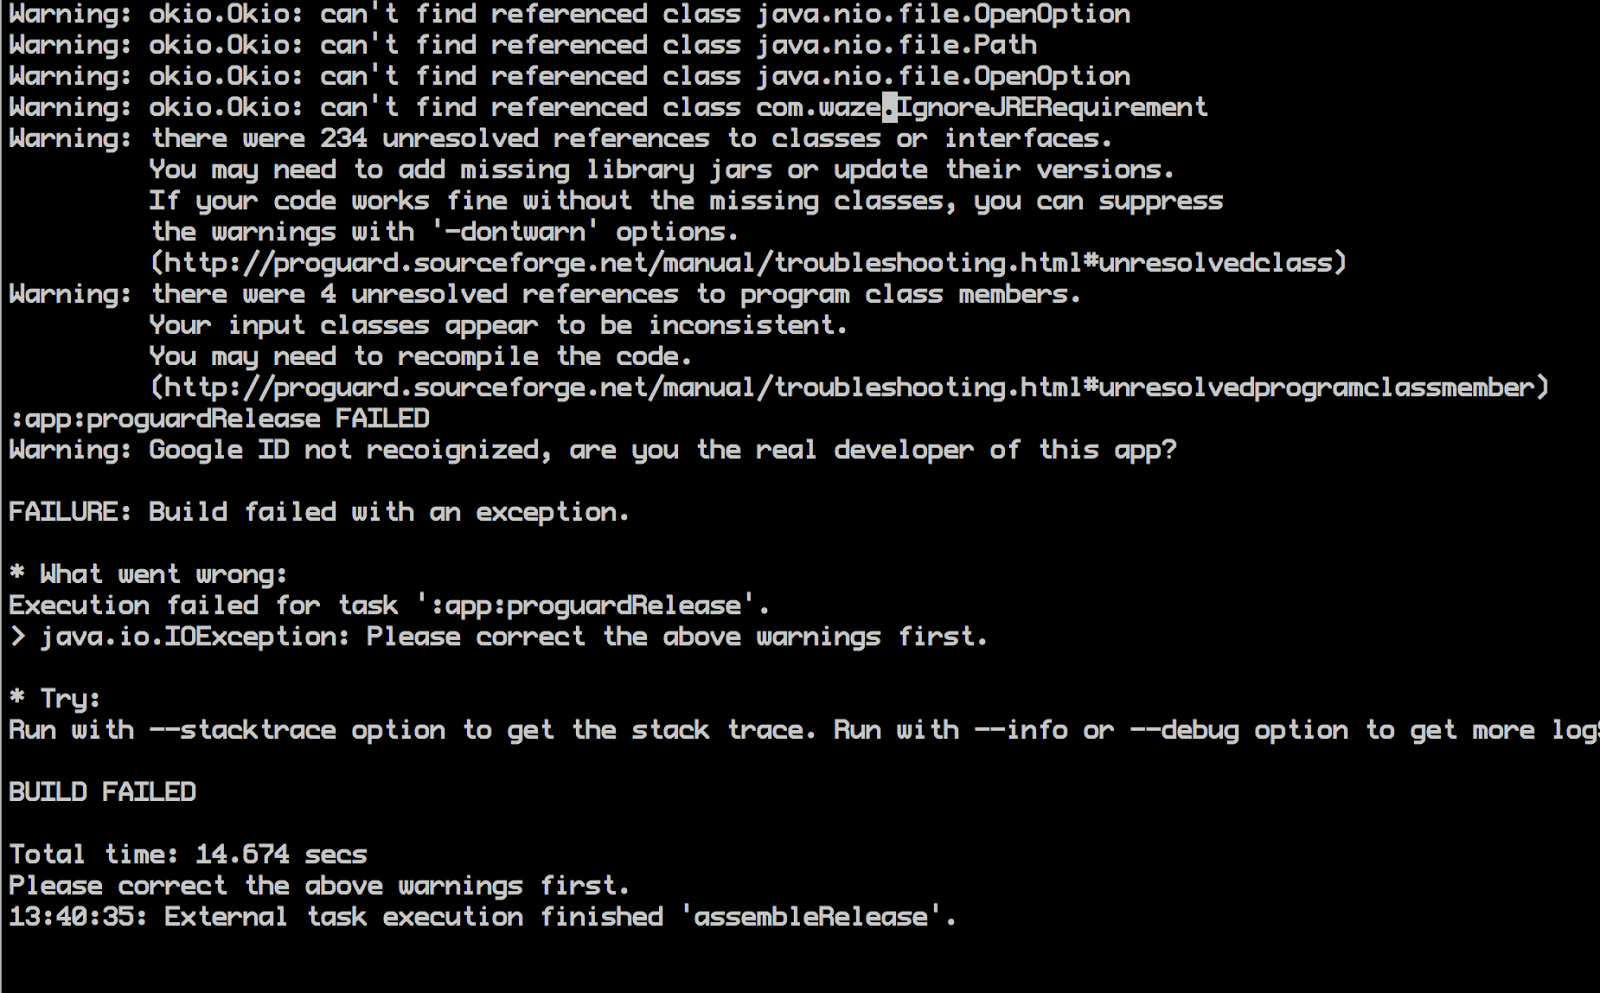
\includegraphics[width=0.6\textwidth]{imagenes/fig25.png}
    \caption{Error al intentar cambiar imagen}
  \end{center}
\end{figure}
%FALTA COMPLETAR LO QUE ES PROGUARD

\section{Decompilación de la aplicación}
Los archivos APK, que son archivos instalables en Android que viene de la sigla Application Package es una variante de los ficheros JAR, de Java Archive, que es un paquete que contiene los archivos necesarios para instalar o hacer correr una aplicación Java.
\\\\
A su vez, un JAR es comparable a un ZIP pero la mayoría de las veces viene sin compresión.
\\\\
    Además, Java, el lenguaje de programación de las aplicaciones Android, es un lenguaje que se compila a bytecode, que es un intermediario entre código de máquina y binario. Este bytecode se hace correr sobre una máquina virtual Java.
\\\\
Finalmente, esto quiere decir que Java es precompilado o preparado para correr más rápido sobre una máquina virtual de Java y gracias a esto es posible lograr programas multiplataforma. Basta con generar una máquina virtual para otro sistema y el programa ya debería correr.
\\\\
El problema de esto es que la capacidad de poder realizar ingeniería inversa es mayor, como el código es intermedio, es más cercano a lo que se programó originalmente.
\\\\
El software APK Studio permite realizar esta ingeniería inversa y generar el árbol de directorios y los instructivos de Java en Smali. Smali es otra forma de decir Assembly (Assembler)
    
        \begin{figure}[H]
  \begin{center}
    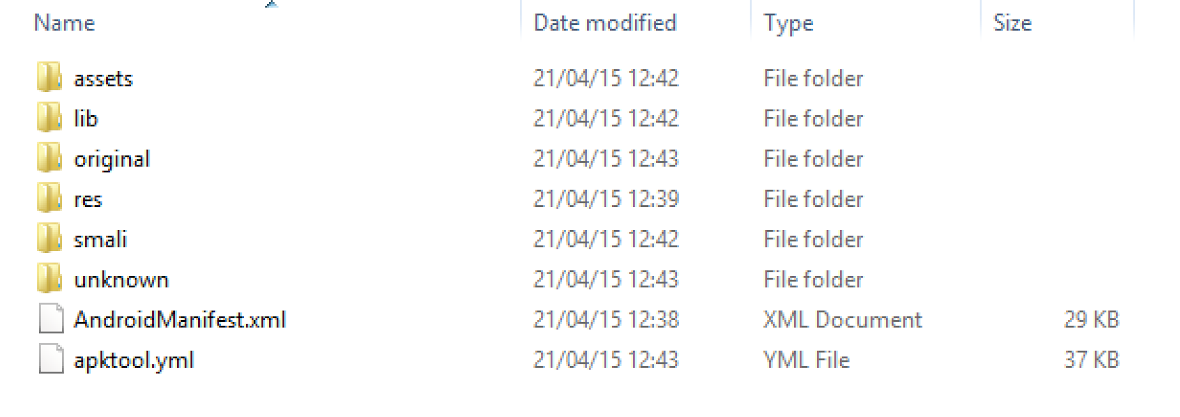
\includegraphics[width=0.9\textwidth]{imagenes/fig26.png}
    \caption{Decompilación del APK Studio}
  \end{center}
\end{figure}
    
En la figura 3 podemos ver la descompilación que realizó APK Studio. En Assets y RES se encuentran las imágenes de la aplicación, en Original encontramos los manifiests (archivos de configuración de muestra de la aplicación en android).
\\\\
Dentro de Smali/com/waze encontramos los assembly de los diferentes trozos de código.
\\\\
Como queremos un código más entendible, transformamos Smali a Java con smali2java ([7]).


    \begin{figure}[H]
  \begin{center}
    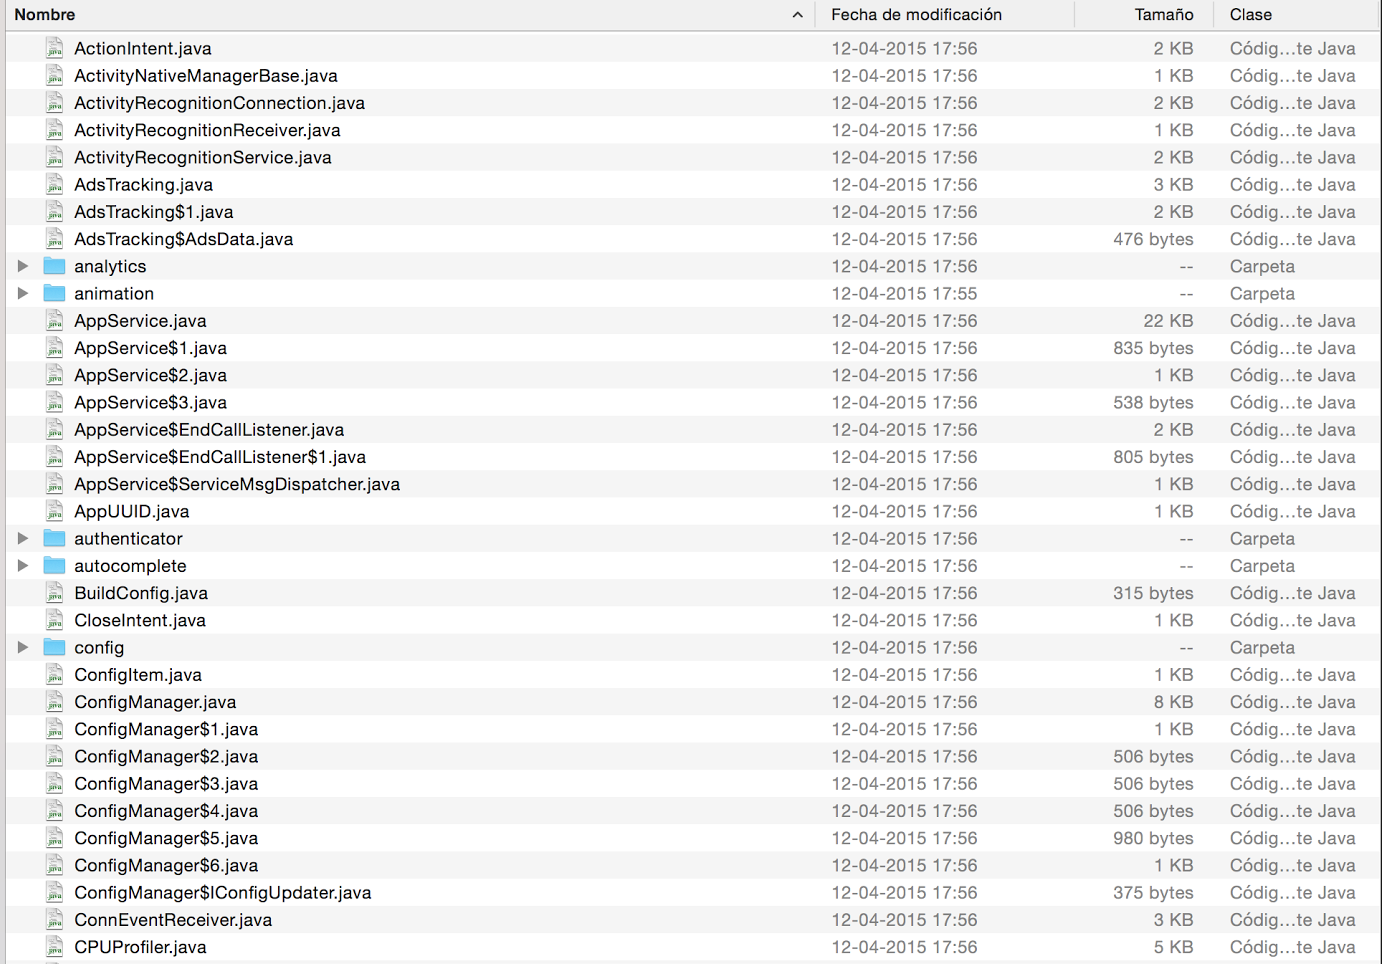
\includegraphics[width=0.9\textwidth]{imagenes/fig27.png}
    \caption{Archivos Smali convertidos a Java}
  \end{center}
\end{figure}

En la figura 4 ya tenemos el código convertido en Java. Aprovechando esto, primero buscamos alguna referencia de alguna base de datos:

    \begin{figure}[H]
  \begin{center}
    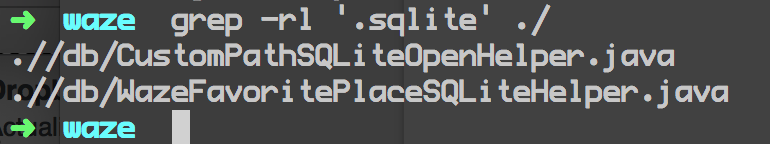
\includegraphics[width=0.8\textwidth]{imagenes/fig28.png}
    \caption{Busqueda de referencia de una base de datos}
  \end{center}
\end{figure}

En el primer archivo (Figura 5) solo hay configuración de la aplicación para utilizar una ruta específica para el fichero SQLite y en el segundo, encontramos una sentencia SQL:

    \begin{figure}[H]
  \begin{center}
    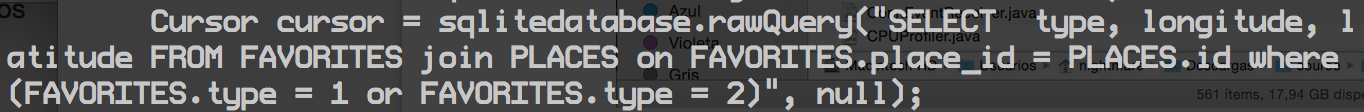
\includegraphics[width=0.8\textwidth]{imagenes/fig29.png}
    \caption{Sentencia sql}
  \end{center}
\end{figure}

En la figura 26 podemos ver que las ubicaciones favoritas (función de Waze) se guarda en el archivo SQLite.
\\\\
Comenzamos la búsqueda de direcciones pero notamos que las direcciones comienzan con “waze://”, esto en una aplicación quiere decir que se definió un esquema único para la aplicación (Esto es, que desde cualquier otra aplicación o navegador, se puede ejecutar Waze mediante una URL ( [9]).

    \begin{figure}[H]
  \begin{center}
    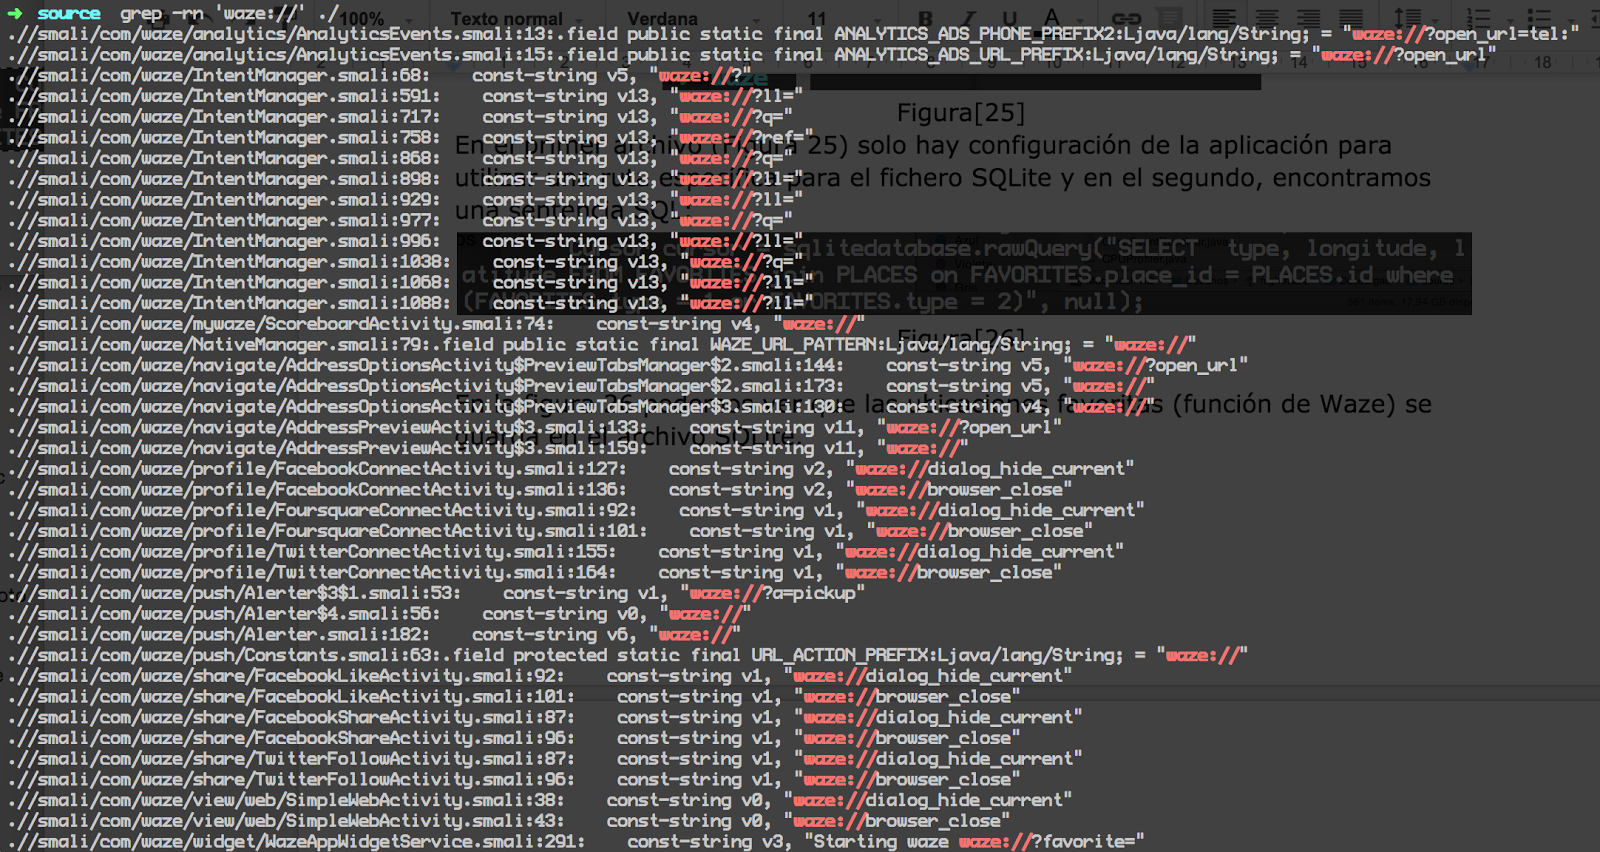
\includegraphics[width=0.9\textwidth]{imagenes/fig30.png}
    \caption{Busqueda de direcciones que comienzan con “waze://”}
  \end{center}
\end{figure}

Investigando, las aplicaciones deben realizar una instanciación de la clase Intent para modificar el comportamiento con una URL específica de una aplicación.
\\\\
Los ficheros de IntentManager encontramos lo siguiente:

    \begin{figure}[H]
  \begin{center}
    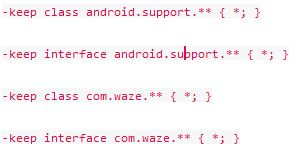
\includegraphics[width=0.8\textwidth]{imagenes/contFig30.JPG}
    \caption{Cotenido de los ficheros de IntentManager}
  \end{center}
\end{figure}


Lo que quiere decir que utilizaron técnicas de ofuscación de código para ocultar la URL original.
\\\\
La ofuscación de código se utiliza para justamente ocultar partes del código sensibles, forzando a que sean compiladas en el momento de crear el APK.
\\\\
En toda solicitud URL hay ofuscación de código. ([8]).


\section{Técnicas de seguridad dentro del código}
\begin{itemize}
\item Waze utiliza archivos Smali que contienen funciones de confidencialidad de la información de cada usuario como son los mensajes por chat, mantener privacidad ubicación del usuario y sus datos personales, y que estos viajen encriptados y que sea difícil obtener ésto en  texto plano.
\item Hay código ofuscado con  proguard.
\end{itemize}





\section{Ataques anteriores a Waze}
\subsection{Estudiantes Israelíes}

En abril del 2014, 2 estudiantes de ingeniería de software llamados Shir Yadid y Meital Ben-Sinaí del Instituto de Tecnología de Israel, como proyecto de su carrera, crearon su propio software. La función de este software consistía en simular un gran taco en una carretera importante de Israel, para desviar el tráfico por carreteras alternativas, pero teniendo en cuenta que esto podría haber provocado un gran caos fue hecho experimentalmente en una de las calles secundarias de su campus.
Este experimento se compuso de las siguientes etapas según cuentan los estudiantes  ([5],[6]):
\\\\
\begin{itemize}
\item Primera etapa: Crear dispositivos móviles con android falsos con un emulador de android. 
\item Segunda etapa: un sistema de control que simulara la intervención humana en el dispositivo que incluía la creación de una cuenta, iniciar sesión y hacer uso de las funciones de Waze. Esto provocó muchos usuarios “wazers” falsos operando.
\item Tercera etapa: Analizar la densidad del tráfico.
\end{itemize}

Luego de éste trabajo, los estudiantes lo notificaron a los desarrolladores de Waze sobre la vulnerabilidad encontrada.


\subsection{¿Está resuelta esta vulnerabilidad?}

Para comprobarlo, realizamos el mismo ataque. Creando 3 máquinas virtuales con Android 4.4 (aprovechando el proyecto Android X86 [8]) instalamos Waze en cada máquina y realizamos un seguimiento de lo que informa Waze en una misma calle.
\\\\
La instalación de Waze en la máquina virtual fue exitosa y además pudimos verificar la cuenta, pero al momento de cargar el mapa no se pudo, dado al problema de GPS con el cual no se cuenta en la máquina virtual y además alertar en cualquier ubicación fue imposible:



        \begin{figure}[H]
  \begin{center}
    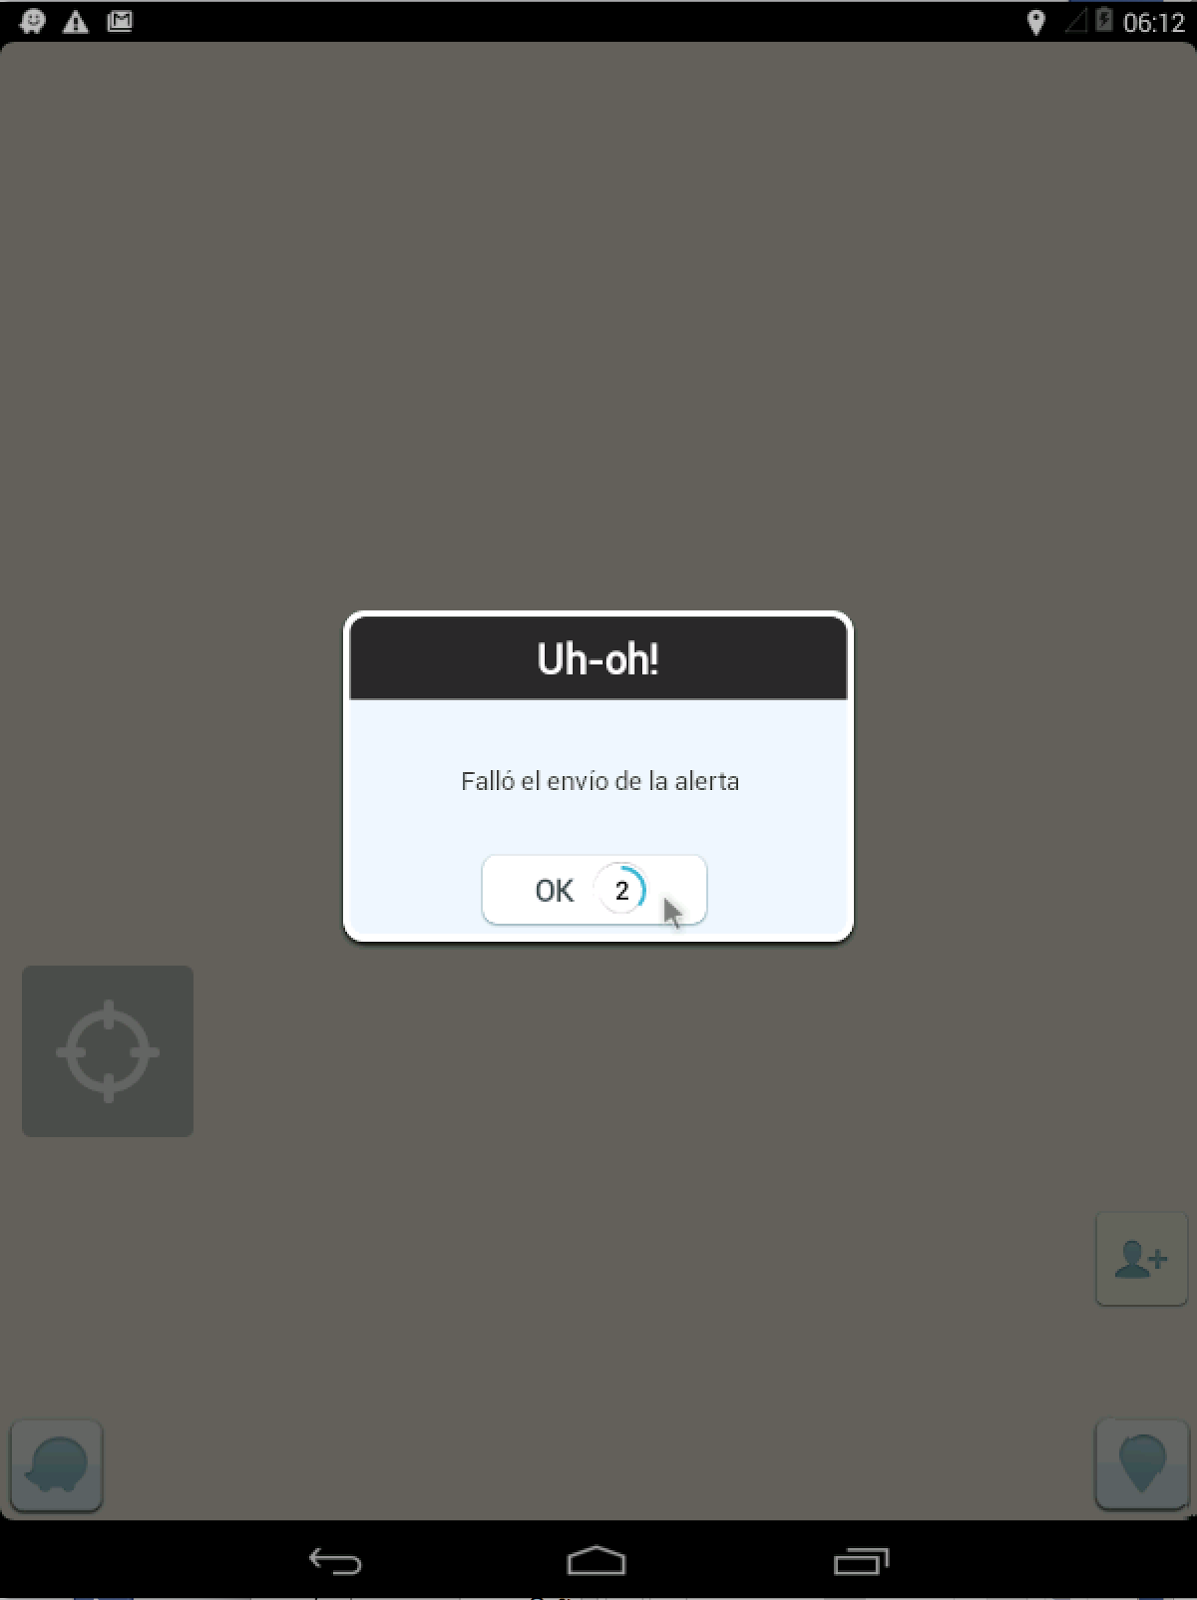
\includegraphics[width=0.4\textwidth]{imagenes/fig18.png}
    \caption{Notificación de Waze de fallo de enviar alerta}
  \end{center}
\end{figure}

Para comprobar si Waze discrimina por información del OS (Android posee un archivo donde guarda la información de la versión del Sistema Operativo), modificamos el archivo /system/build.prop con la misma configuración del teléfono móvil:

    
            \begin{figure}[H]
  \begin{center}
    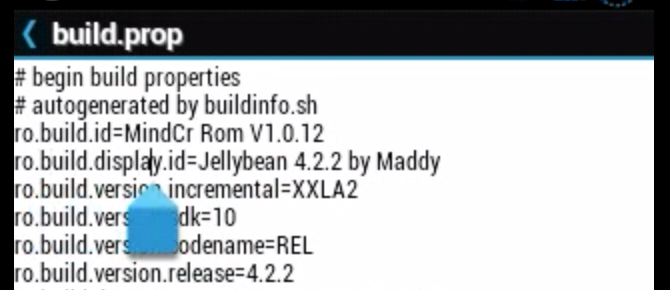
\includegraphics[width=0.9\textwidth]{imagenes/fig19.png}
    \caption{Archivo buld.prop}
  \end{center}
\end{figure}
    
De todas maneras no fue posible enviar una alerta desde una máquina virtual.
\\\\
De manera alterna, se intentó alertar con más de un dispositivo móvil una misma ubicación. Al parecer, si el usuario Waze no ha pasado por la ubicación o no se encuentra cerca, su alerta se recibe pero no se hace válida. En nuestro caso, uno de nosotros desde el sector oriente de Santiago realizó una alerta en el sector sur, La Florida, de tráfico denso. Esta alerta no apareció en la aplicación, pero al alertar cerca de la ubicación apareció inmediatamente en ambos dispositivos.
    
  
    
   \begin{figure}[H]
  \begin{center}
    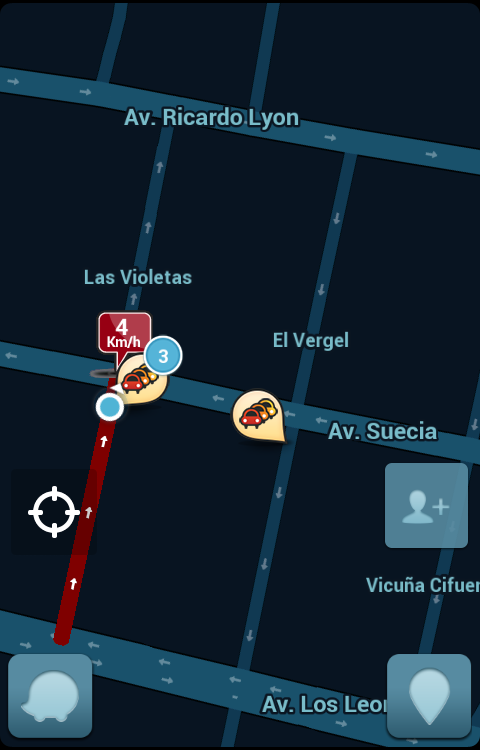
\includegraphics[width=0.5\textwidth]{imagenes/fig20.png}
     \caption{Envío de altertas ubicación 1, dispositivo 1}
  \end{center}
\end{figure}


        \begin{figure}[H]
  \begin{center}
    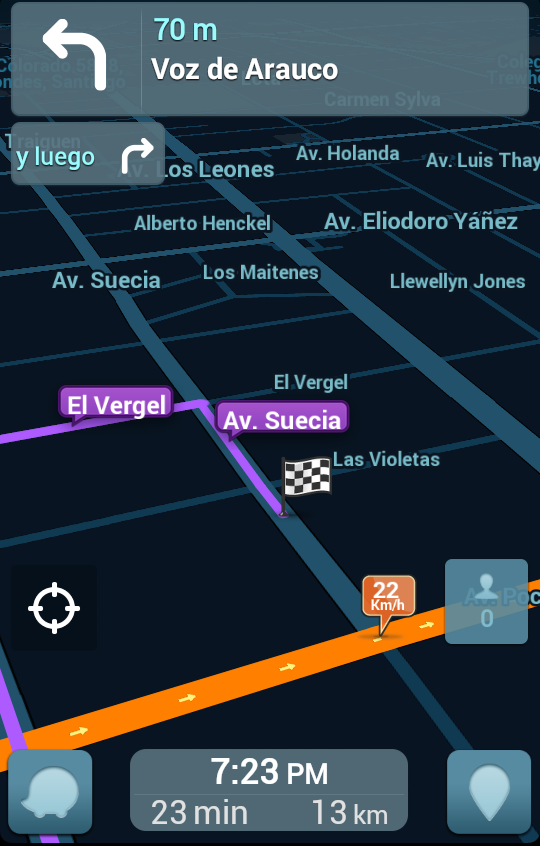
\includegraphics[width=0.5\textwidth]{imagenes/fig21.png}
     \caption{Vista del punnto de envío de las alertas por el dispositivo 1, en el                   dispositivo 2}
  \end{center}
\end{figure}
    
En la figura 11, se muestran 3 envíos seguidos, realizados de alerta de tráfico detenido, desde un dispositivo móvil. Estas alertas fue posible enviarlas por la ubicación del dispositivo, que era cercana a la calle.
\\\\
En la figura 20, desde otro dispositivo no vemos que haya tráfico en la misma dirección.


        \begin{figure}[H]
  \begin{center}
    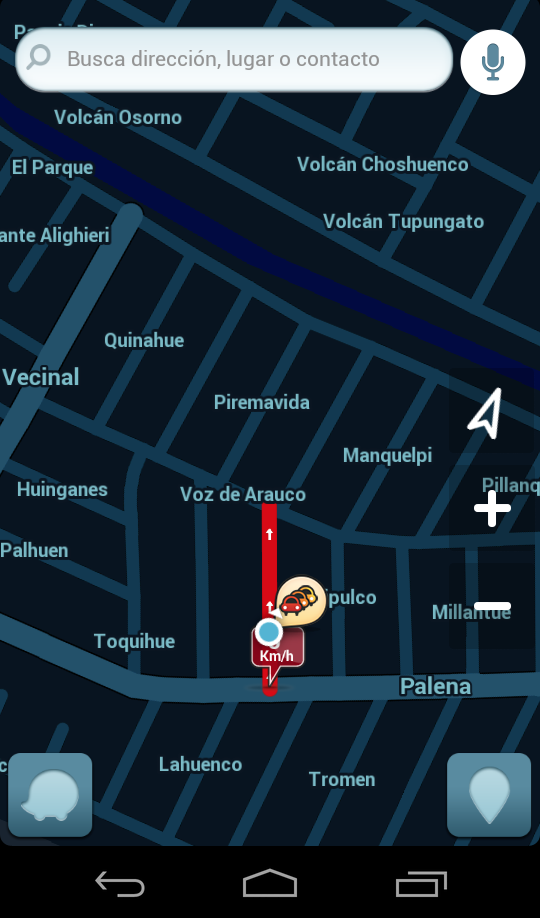
\includegraphics[width=0.5\textwidth]{imagenes/fig22.png}
    \caption{Envíos de alerta en el dispositivo 2}
  \end{center}
\end{figure}


        \begin{figure}[H]
  \begin{center}
    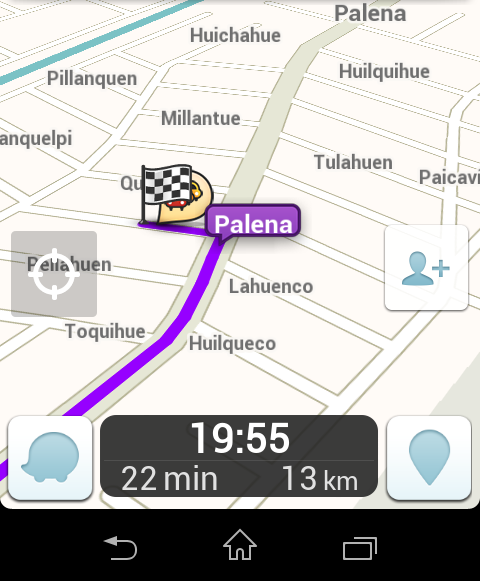
\includegraphics[width=0.5\textwidth]{imagenes/fig23.png}
    \caption{Vista del punnto de envío de las alertas por el dispositivo 2, en el                   dispositivo 1}
  \end{center}
\end{figure}


En caso contrario, usando un usuario frecuente en Waze se hizo la alerta en una calle cercana a la ubicación del dispositivo con ese usuario y con el otro dispositivo si se pudo ver la alerta.
\\\\
En Waze, los usuarios ganan puntos a medida que utilizan la aplicación, a medida que utilizan el mapa, conducen, generan acciones con la aplicación se gana puntaje. [1]
\\\\
Para este ejemplo, el usuario frecuente tiene el ranking de Waze Loyalty, los cuales son los usuarios pertenecientes al 1% de los puntajes más altos de Chile contra un Waze Baby que no ha recorrido más de 100 millas para ascender a otro nivel.
\\\\
Con estas pruebas se comprueba que los desarrolladores de Waze corrigieron la vulnerabilidad encontrada por los estudiantes israelíes.

\section{Función Indent (Direcciones waze://)}
Como se dijo en la etapa de descompilado, Waze utiliza direcciones únicas para sus consultas y esta dirección puede ser utilizada por otras aplicaciones para ejecutar Waze con algún comando.
\\\\
Analizando los ejemplos para desarrolladores, una forma de invocar Waze es con la dirección “waze://q=” y concatenando la búsqueda y esto genera una búsqueda dentro de Waze tal como si el usuario la buscara.
\\\\
Por tanto, se probó en un sitio HTML que invocara la url “waze://q=Facultad de Ingeniería UDP, Chile Santiago” (http://output.jsbin.com/telecozazi) para que ejecutara Waze con esa búsqueda.

        \begin{figure}[H]
  \begin{center}
    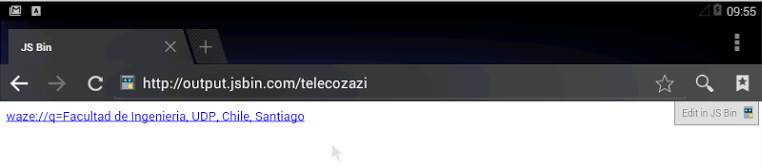
\includegraphics[width=0.3\textwidth]{imagenes/fig43.png}
    \caption{Sitio HTML que invoca url waze://}
  \end{center}
\end{figure}


Al abrir el enlace en el navegador de Android se ejecutó Waze generando la búsqueda dicha.

        \begin{figure}[H]
  \begin{center}
    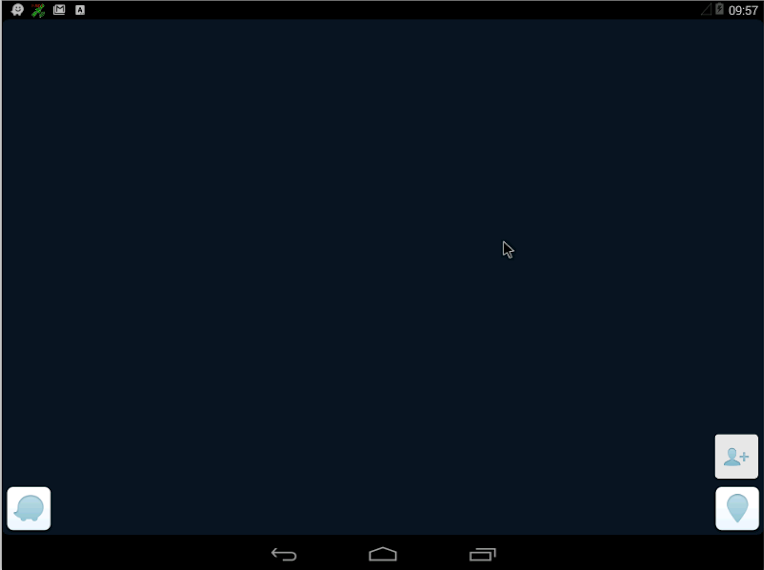
\includegraphics[width=0.3\textwidth]{imagenes/fig44.png}
    \caption{Ejecución de Waze al abrir la url Waze:// en la imagen anterior}
  \end{center}
\end{figure}


El mapa, no se muestra debido a que Waze de alguna manera detecta los programas que establecen ubicaciones que no corresponden, pero si realizó la acción solicitada.


\section{Modificación y eliminación de paquetes}
No fue posible modificar o alterar la interacción con el servidor de Waze dado que el protocolo está ofuscado y no podemos realizar auditoría al respecto. 
\\\\
De todas formas, se alteró el comportamiento de la conectividad de Waze  utilizando IPTables para ver su comportamiento.
\\\\    
Con IPTables, al momento de realizar una petición de rutas en Waze (colocando una dirección a la cual queremos llegar), añadimos una regla que votara todo tráfico proveniente que tuviera la IP con la cual nuestra APP se había estado comunicando:
\\\\
iptables -A INPUT -s 65.55.44.100 -j DROP
\\\\
Estos argumentos en IPTables indican que debe ser añadida una regla para los paquetes de entrada (INPUT) desde el origen (-s) 65.55.33.100 con la acción DROP (votar el paquete).

            \begin{figure}[H]
  \begin{center}
    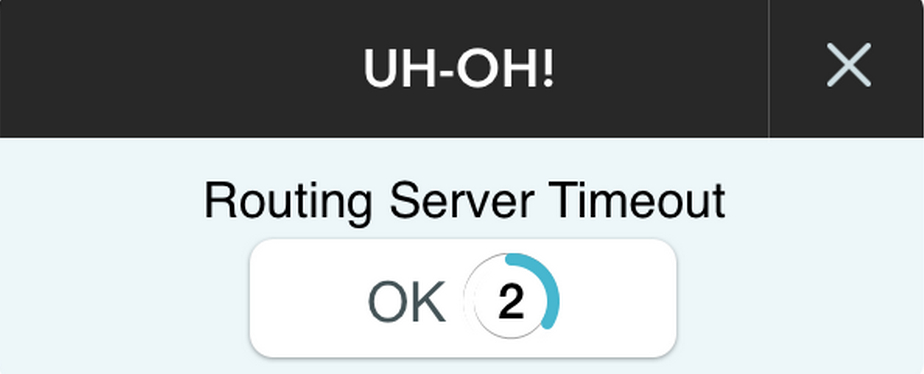
\includegraphics[width=0.3\textwidth]{imagenes/fig45.png}
    \caption{Error de conexión a internet}
  \end{center}
\end{figure}
    
    
Waze al no recibir los paquetes de respuesta de la solicitud de ruteo nos advierte que esperó al servidor de rutas pero este no le respondió [Figura 17].
\\\\
De manera similar, se hizo para cuando se hizo una alerta de tráfico en Waze, al seleccionar que había mucho tráfico en nuestra ubicación, se realizó el mismo comando con IPTables.

        \begin{figure}[H]
  \begin{center}
    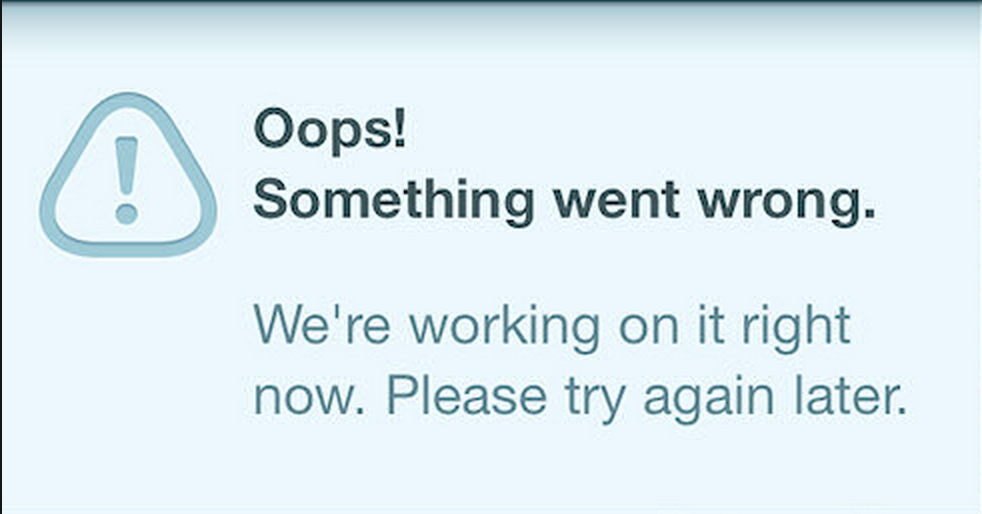
\includegraphics[width=0.3\textwidth]{imagenes/fig46.png}
    \caption{Error generado al ser modificado previamente un servidor DNS en el dispositivo}
  \end{center}
\end{figure}


Waze nos advierte que hay un error, pero esta vez no nos indica de qué se trata. Podría ser una excepción no rescatada dentro del código (Figura[18]).


\section{Funcionalidad en maquina virtual}
En VirtualBox, aunque se instalamos más de una aplicación como fake gps (figura 17):


        \begin{figure}[H]
  \begin{center}
    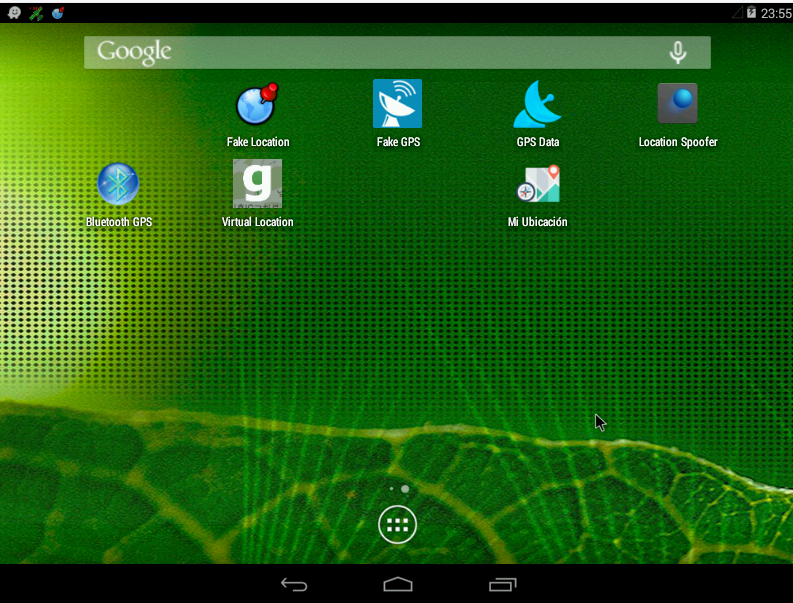
\includegraphics[width=0.6\textwidth]{imagenes/fig31.png}
    \caption{Aplicaciones instaladas para fakegps}
  \end{center}
\end{figure}


Waze no mostró el mapa, como se ve en la figura 20:

        \begin{figure}[H]
  \begin{center}
    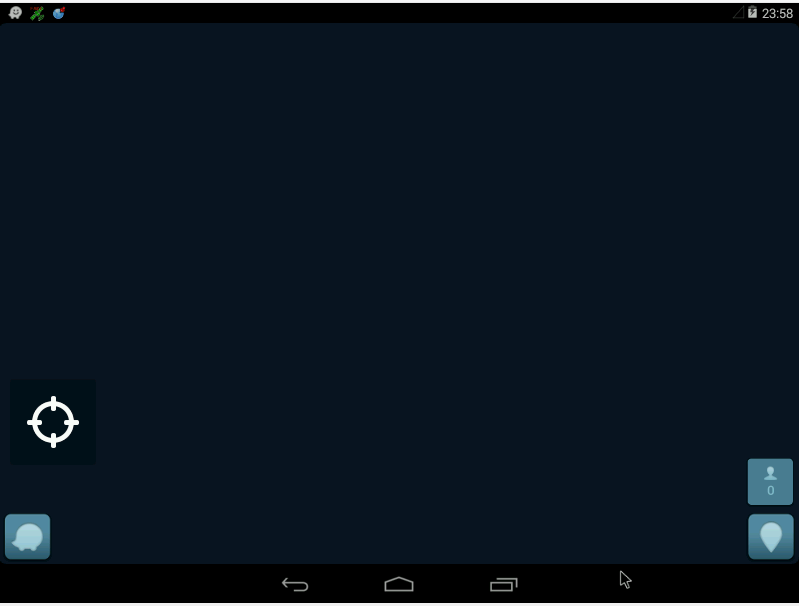
\includegraphics[width=0.6\textwidth]{imagenes/fig32.png}
    \caption{Waze no muestra mapa en maquina virtual (VirtualBox) }
  \end{center}
\end{figure}

En la máquina virtual al enviar una alerta, no aparece el mensaje de alerta enviada, figura 19:

        \begin{figure}[H]
  \begin{center}
    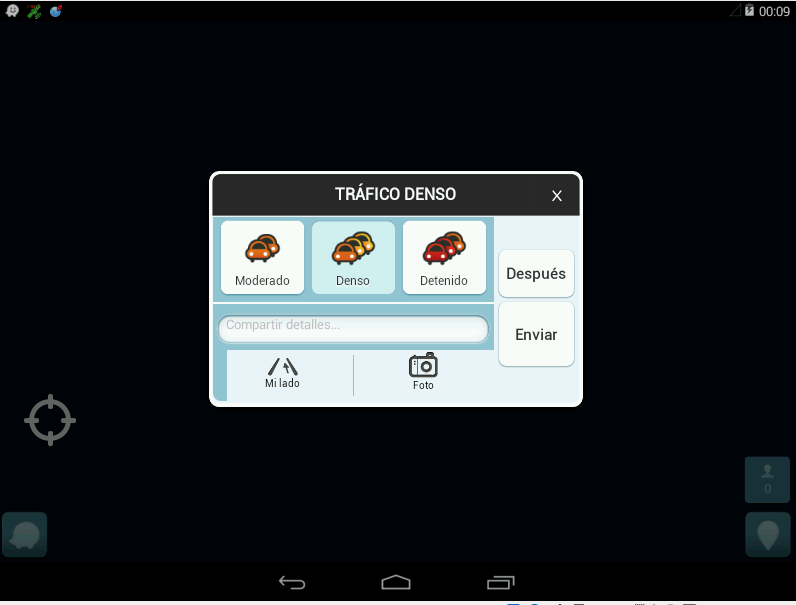
\includegraphics[width=0.6\textwidth]{imagenes/fig33.png}
    \caption{En la maquina virtual no se muestra el mensaje de alerta enviada}
  \end{center}
\end{figure}

Como es el caso de enviar una alerta desde un celular:

        \begin{figure}[H]
  \begin{center}
    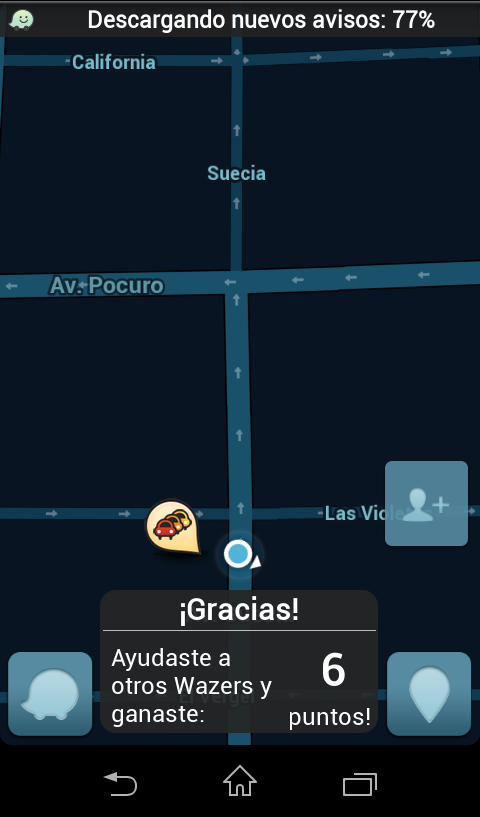
\includegraphics[width=0.3\textwidth]{imagenes/fig34.png}
    \caption{Mensaje de alerta enviada mostrada en un celular}
  \end{center}
\end{figure}

Otra opción descartando VirtualBox, fue probar con el emulador de android BlueStacks:

        \begin{figure}[H]
  \begin{center}
    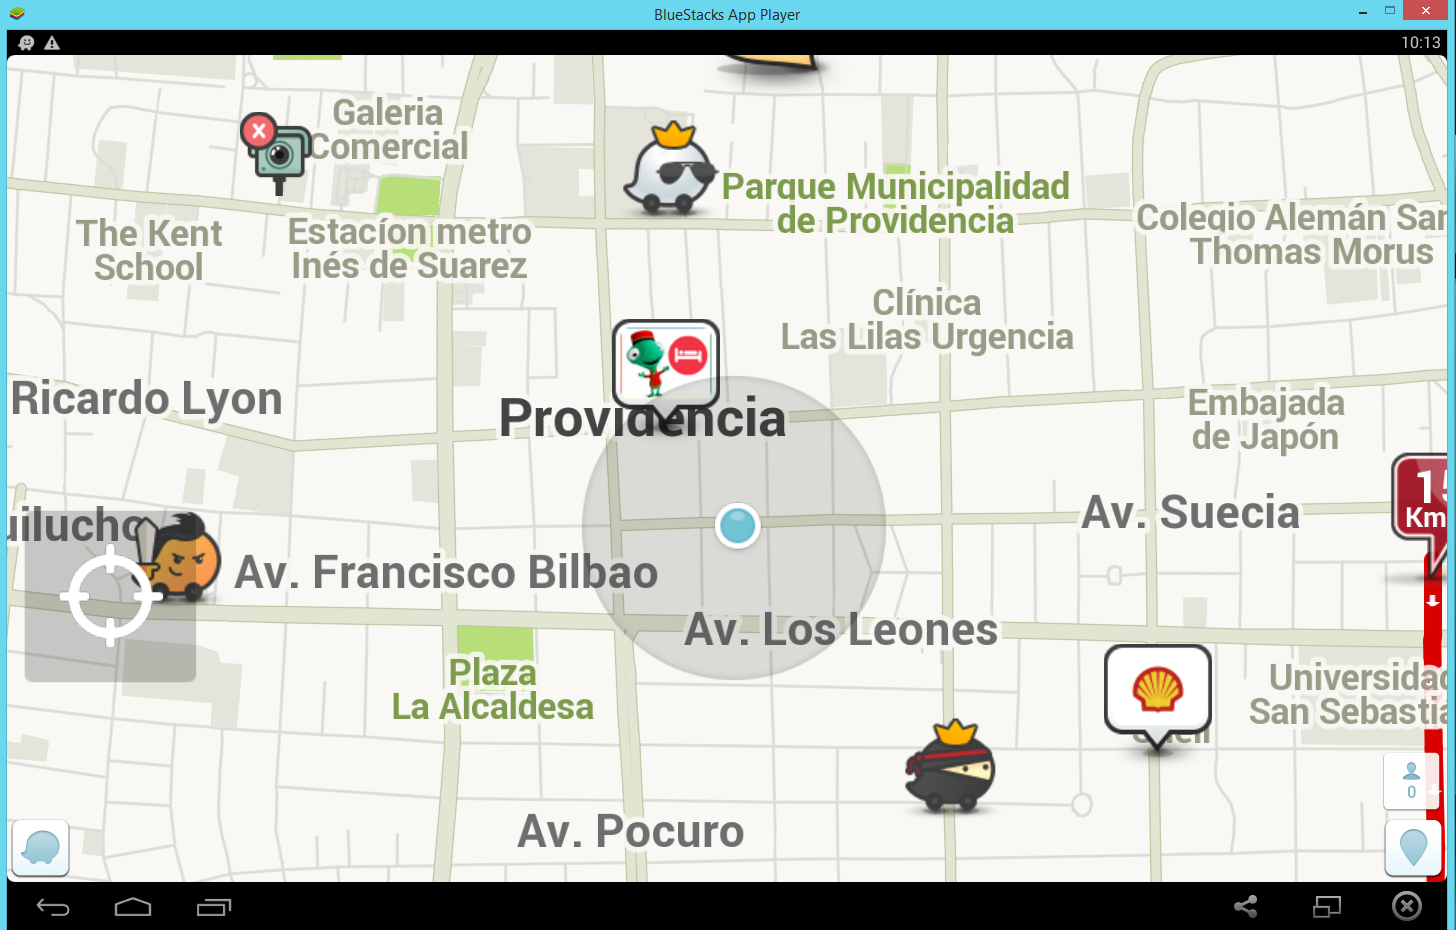
\includegraphics[width=0.7\textwidth]{imagenes/fig35.png}
    \caption{Waze en el emulador de Android Bluestacks}
  \end{center}
\end{figure}

En este caso si se muestra el mapa, y también es posible enviar una alerta:

        \begin{figure}[H]
  \begin{center}
    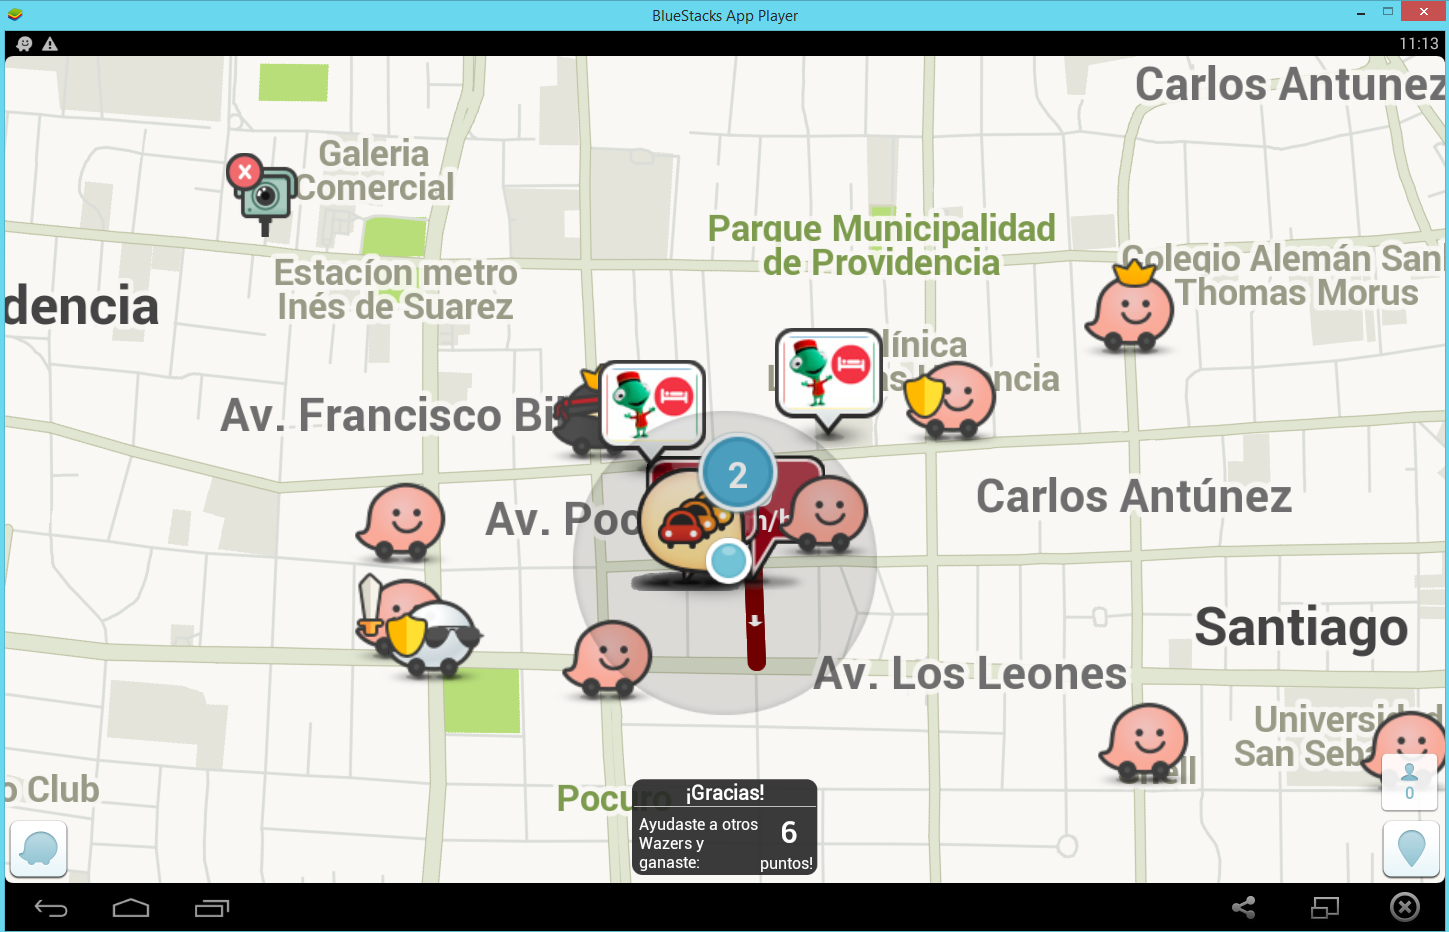
\includegraphics[width=0.7\textwidth]{imagenes/fig36.png}
    \caption{En Bluestack, Waze si muestra el mapa como en un celular}
  \end{center}
\end{figure}


y luego de enviarla aparece en el celular:

        \begin{figure}[H]
  \begin{center}
    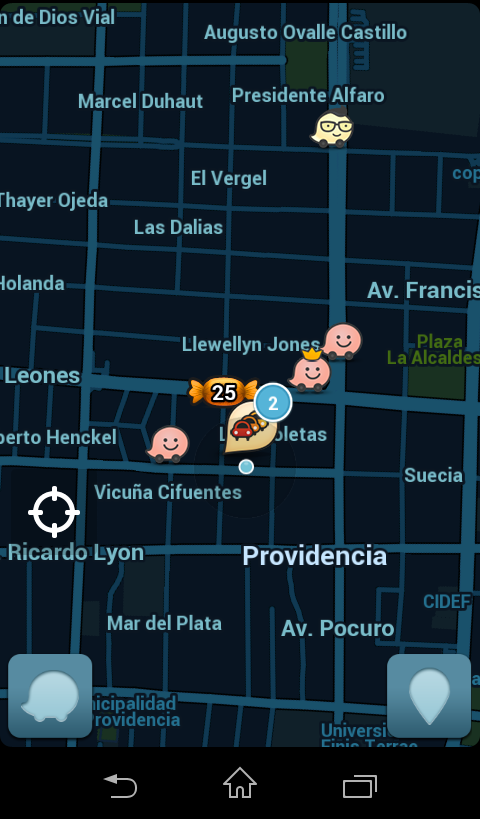
\includegraphics[width=0.3\textwidth]{imagenes/fig37.png}
    \caption{Alerta enviada usando Bluestacks aparece se muestra en un celular}
  \end{center}
\end{figure}

El problema que encontramos con BlueStacks fue que no es posible acceder a los archivos de la aplicación desde afuera. Pero si en la máquina virtual de Android:

        \begin{figure}[H]
  \begin{center}
    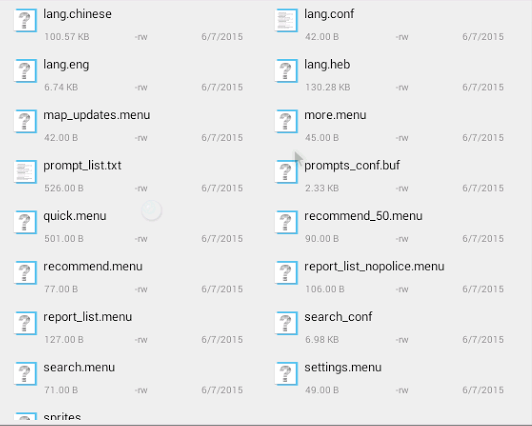
\includegraphics[width=0.7\textwidth]{imagenes/fig38.png}
    \caption{Archivos de Waze dentro de la maquina virtual}
  \end{center}
\end{figure}

        \begin{figure}[H]
  \begin{center}
    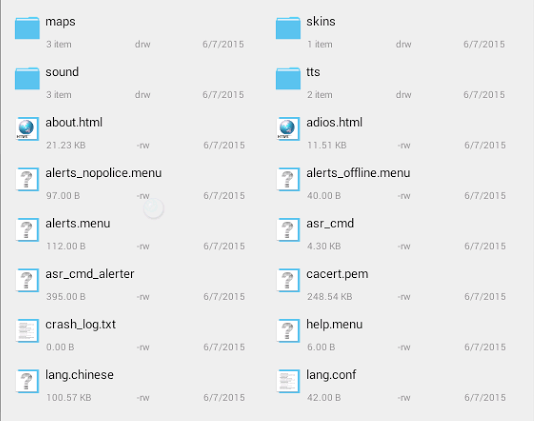
\includegraphics[width=0.7\textwidth]{imagenes/fig39.png}
    \caption{Más archivos de Waze dentro de la máquina virtual}
  \end{center}
\end{figure}

Dentro de los archivos no se encontró nada configurable. El archivo lang.conf solo mantenía los nombres de los lenguajes disponibles del software. [Figura 26 y 27]

En los archivos menús al parecer mantiene llamadas a funciones de Waze, ya que solo mantiene líneas con nombres de acciones aparentemente. [Figura 26]

        \begin{figure}[H]
  \begin{center}
    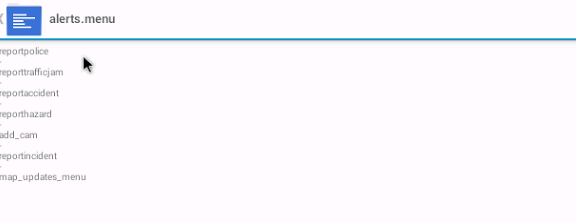
\includegraphics[width=0.9\textwidth]{imagenes/fig40.png}
    \caption{Contenido archivo alerts.menu}
  \end{center}
\end{figure}

De todas formas, intentamos modificar para ver si esto tiene incidencias en la aplicación, modificando el mismo archivo de alertas con uno similar:


        \begin{figure}[H]
  \begin{center}
    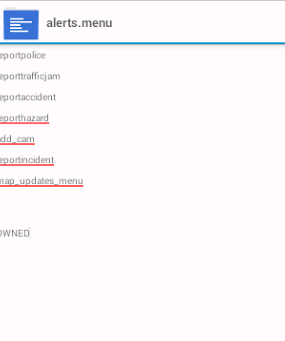
\includegraphics[width=0.6\textwidth]{imagenes/fig41.png}
    \caption{Archivo alerts.menu modificado}
  \end{center}
\end{figure}

Pero esto no tuvo repercusiones en la aplicación:


        \begin{figure}[H]
  \begin{center}
    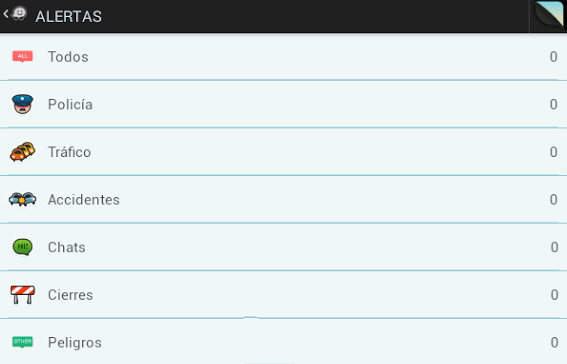
\includegraphics[width=0.6\textwidth]{imagenes/fig42.png}
    \caption{Menu de alertas no es afectado por la modificación del archivo alerts.menu}
  \end{center}
\end{figure}


Se volvió a verificar la aplicación y esta había reemplazado el archivo alerts.menu con el archivo original, por tanto, podemos deducir que la aplicación genera estos ficheros al iniciar.



\section{Conclusiones}
Waze resulta ser una aplicación muy robusta y con buenas prácticas en su codificación. 
\\

Las buenas prácticas de seguridad deben ser un punto fuerte en el desarrollo de cualquier tipo de software y más aún cuando deben ser programados en lenguajes descompilables como Java, donde no se tiene otra opción. Si no se toman medidas en cuanto a la comunicación de la aplicación y técnicas de ofuscación es muy probable que usuarios con malas intenciones generen aplicativos que roben información o alteren el flujo normal de la misma.





\end{document}

